\section{Цель работы}
	Научиться имитировать для компонента распределенной системы его окружение и воздействия для нужд построения автоматических тестов.
		
\section{Порядок выполенения работы}
	\subsection{Генерация заготовок тестов}
		\begin{figure}[h]
			\centering
			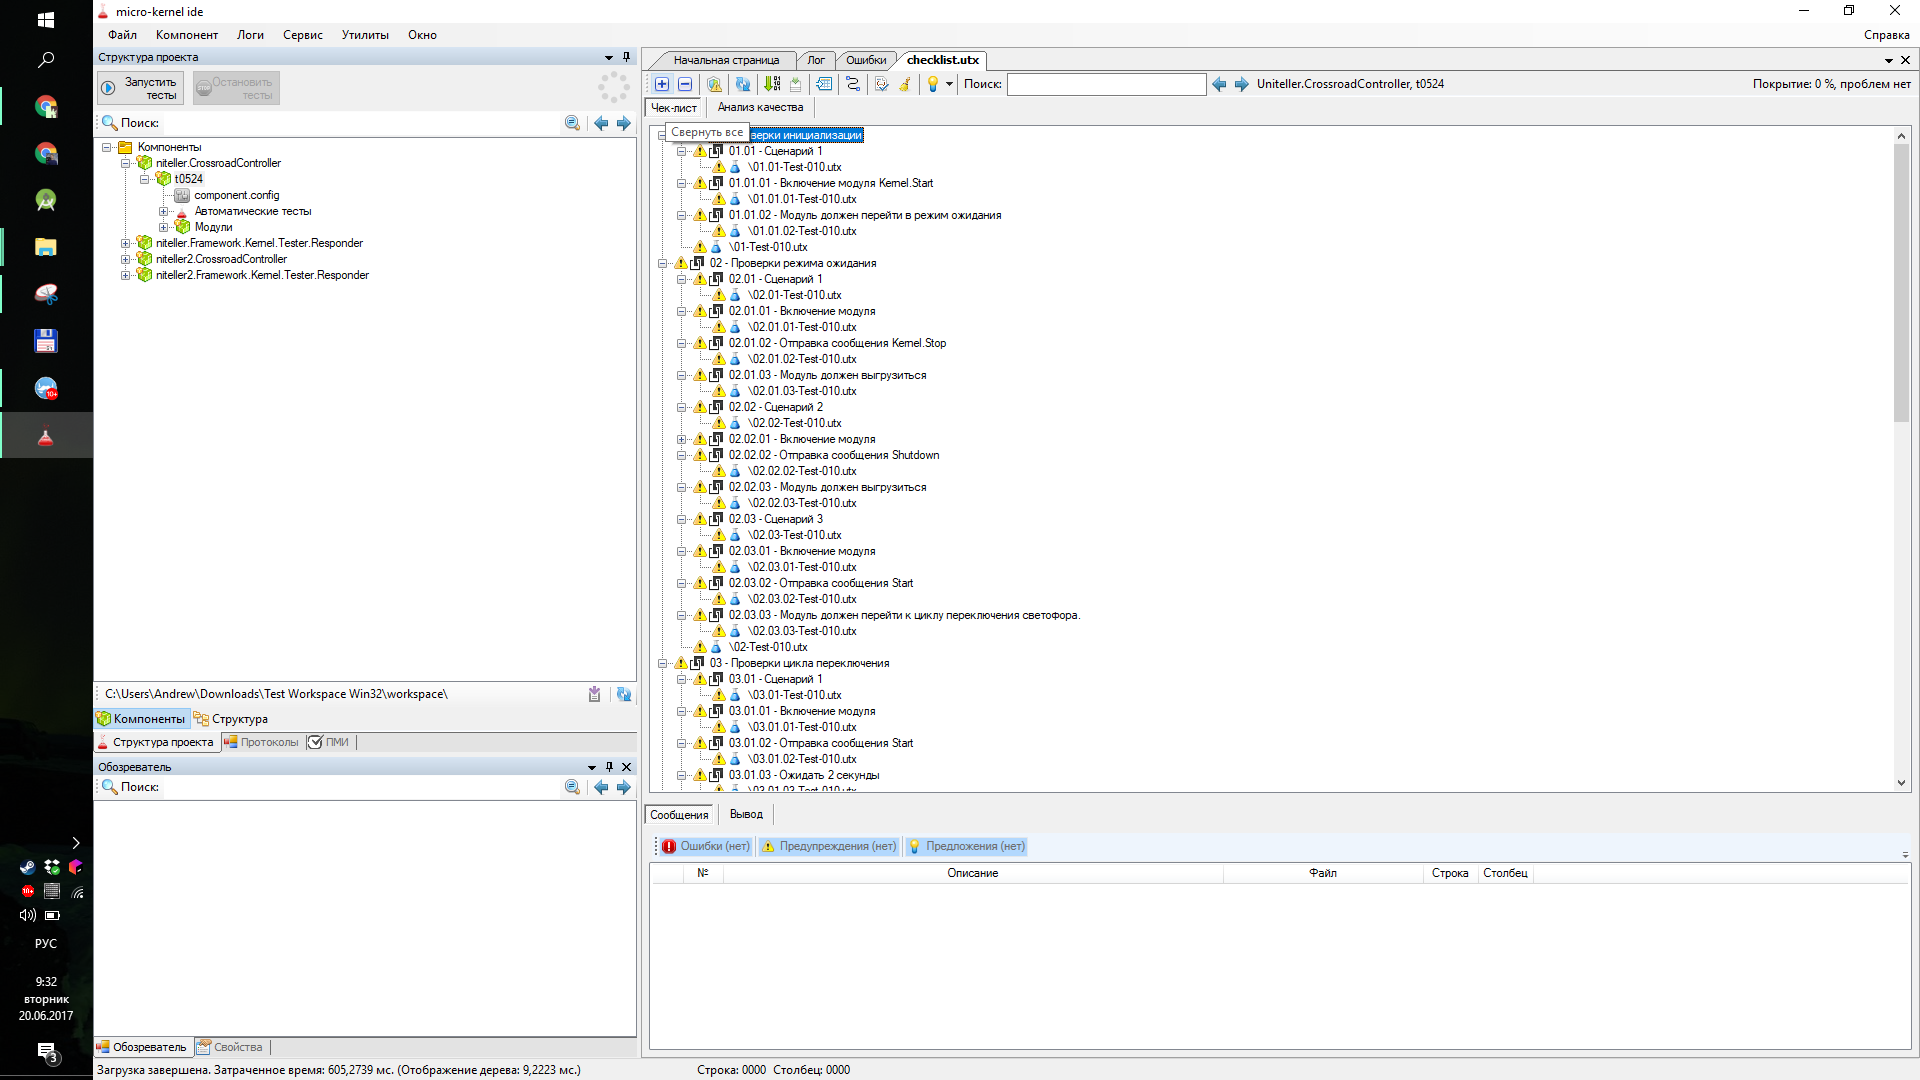
\includegraphics[width=\linewidth]{images/tests}
			\caption{Сгенерированные заголовки тестов}
			\label{fig:tests}
		\end{figure}
		
	\newpage
	\subsection{Реализовать автоматический тест}
		\lstinputlisting[caption={Реализация теста проверки смены состояния}]{listings/test.utx}
		
\section{Вывод}
	Для компонента распределенной системы сымитировано его окружение и построен автоматический тест.